\section{Introduction}
\label{sec:intro}


In computer graphics and vision, achieving realistic renderings for intricate surface materials hinges on accurately describing the interaction of light with the surfaces. This is conventionally conveyed through the modelling and reconstruction of a 4D Bidirectional Reflectance Distribution Function (BRDF), which quantifies the relationship between the incident and outgoing light intensities for a specific material. In this chapter, I propose a novel generalisable \gls{BRDF} representation model that can estimate the \gls{BRDF}s of new materials from highly sparse and unstructured point-based samples \footnote{Point-based samples refer to the \gls{BRDF} values acquired at specific points on a surface with known viewing and lighting directions.} and compress the densely sampled values into very small latent embeddings.


While there has been prior work that attempts to tackle similar tasks by estimating the free parameters of analytic \gls{BRDF}s or the principal components of \gls{BRDF}s from images or reflectance measurements, the oversimplified models of the complex \gls{BRDF} function lead to inaccuracies when predicting real materials, thereby diminishing the realism in renderings~\cite{ngan2005}. Moreover, the process of fitting through nonlinear optimisation is inherently unstable, computationally expensive, and prone to local minima, hindering the accurate reconstruction of material appearance~\cite{dupuy2015, guarnera2016}. Measured \gls{BRDF}s of real-world materials can also be fraught with errors due to equipment limitations, adding to the complexity of the fitting process~\cite{nielsen2015optimal}. 

\begin{figure}
  \centering
   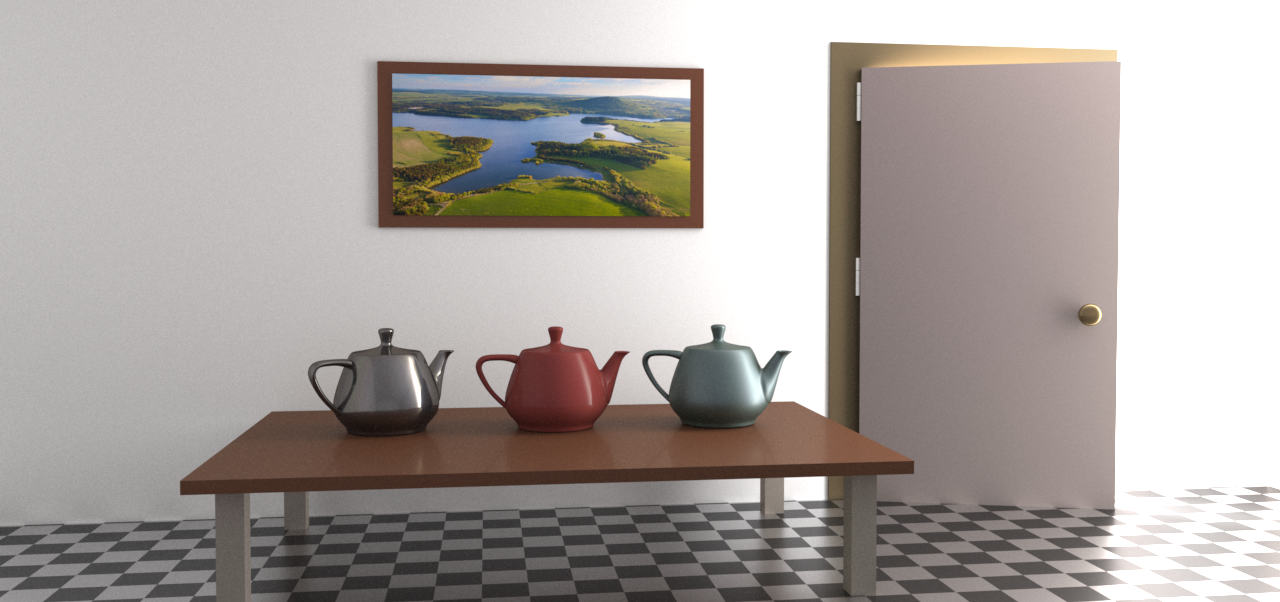
\includegraphics[width=\linewidth]{Chapters/hyperbrdf-figs/teaser_cropped.png}
   \caption{A room scene rendered with materials reconstructed by HyperBRDF, including sparse reconstruction (table top and legs, door, door and picture frames, hinge), compression (two teapots on the left, door handle) and \gls{BRDF} interpolation (right-most teapot). Scene courtesy of [Benedikt Bitterli].}
   \label{fig:teaser}
\end{figure}

Recent advances in deep learning have enabled the accurate representation of complex continuous signals (\textit{e.g.} images, surfaces, volumes, materials, \textit{etc.}) using a Neural Field~\cite{sitzmann2020siren, ffn, cnf2023}, \textit{i.e.} a neural network mapping coordinate inputs to sampled values, without compromising model compactness. Consequently, neural fields have gained substantial popularity for representing continuous \gls{BRDF}s in recent works~\cite{sztrajman2021neural, cnf2023}. However, reconstructing a neural field representation for \gls{BRDF}s typically requires training the network with a regression loss function to overfit to a single material, which demands dense sampling and extensive computational resources, while being unable to generalise to new materials.

More recently, Generalisable Neural Fields~\cite{rebain2022attention} (\gls{GNF}s) have emerged as a promising solution to the aforementioned challenges. Rather than overfitting to individual signals, \gls{GNF}s are designed to learn a generalised mapping, either deterministic or probabilistic, between sampled signals and their full neural field representations in a fashion similar to supervised learning. The key strategy of \gls{GNF}s involves conditioning the neural fields with a latent embedding of the signal samples. Popular conditioning mechanisms include concatenated latent vectors~\cite{park2019deepsdf}, hypernetworks~\cite{ha2017hypernetworks}, and attention-based set latent representations~\cite{jiang2021cotr}. Once the conditional neural field is properly learned, reconstruction of the full signal can be achieved at inference time, and even with highly sparse and unstructured samples.


Inspired by \gls{GNF}s, I propose a novel framework, HyperBRDF, for generalisable neural \gls{BRDF} representation for both the estimation of unseen materials from sparse and unstructured samples and the compression of measured \gls{BRDF}s into low-dimensional latent space. In this framework, I employ a multi-layer perceptron (\gls{MLP}) model as the neural field backbone for \gls{BRDF} representation, a hyper-network for conditioning, and a set encoder that allows for mapping an arbitrary number of reflectance measurements from arbitrary directions to a compact latent embedding for conditional \gls{BRDF} generation. 
The built-in nonlinear interpolation capability of the hyper-network also offers robust and adaptable material editing and blending across various sample sizes.


Unlike previous work, the \gls{BRDF} reconstruction by HyperBRDF is highly efficient without the need for extensive training to overfit individual materials, while also maintaining state-of-the-art performance in reconstruction accuracy for sample size below 4000; see Figure~\ref{fig:imp_comp_upt}.


In summary, HyperBRDF offers a novel solution for the challenging task of generalisable \gls{BRDF} modelling with the following key contributions:
\begin{itemize}
    \item{\textbf{Generalisability and Adaptability:} HyperBRDF ensures robustness and adaptability across varying sample sizes and appearances, making it highly effective for estimating the \gls{BRDF}s of unseen materials from highly sparse and unstructured sampling. Its adaptability also extends to highly compact representation of \gls{BRDF}s, overall outperforming the prior state-of-the-art compression method; see Table \ref{table: oursvsnps}.}
    

    \item{\textbf{Realism and Accuracy:}
    My extensive evaluation demonstrates the superior performance of HyperBRDF in reconstructing the \gls{BRDF}s of 20 test materials from a limited number of samples, ranging from 40 to 4000, outperforming prior methods in terms of appearance modelling and colour preservation (by at least 2dB in peak-signal-to-noise ratio and 1 in Delta E).
    }
\end{itemize}

\section{Motivation and impact}
\label{sec:hyperbrdf-mot}

The representation of measured \gls{BRDF}s is crucial in computer graphics, especially in physically-based rendering (\gls{PBR}) for applications such as filmmaking, gaming, virtual and augmented reality, and product design, aiming for immersive realism. \gls{PBR} provides a more precise portrayal of light-material interactions. However, real-world \gls{BRDF} models are reconstructed by taking samples with a device, such as a camera or gonioreflectometer and often demand numerous samples, making acquisition, storage, and manipulation costly and challenging. For instance, the MERL dataset \cite{Matusik2003jul}, the main dataset I utilised for experiments, captures 330 high dynamic range images with a CCD camera for each material in roughly four hours. The RGL dataset \cite{dupuy2018adaptive}, the secondary dataset included in training, captures samples with a gonioreflectometer that leads to captures times of approximately 2.5 hours for isotropic materials. Therefore, HyperBRDF offers multiple impactful contributions: 
\begin{itemize}
 \item can integrate with professional setups where capturing only one material can take hours. HyperBRDF’s superior sparse reconstruction ability can help significantly reduce the manual and heavy workload of material acquisition. I also discuss the related work aligned with this research line in Section \ref{hyperbrdf-RW}.
 \item Providing \gls{BRDF} compression with high accuracy and efficiency, encoding over a million samples into a 7D latent vector, saving storage space and increasing transfer speed. 
 \item Allowing easy material editing through its latent space representation.
 \end{itemize}
